\subsection{Oddělený překlad, sestavení, řízení překladu}

\subsubsection*{Struktura programu}

Program se skládá z \emph{modulů}:
\begin{pitemize}
	\item Překládány samostatně kompilátorem 
	\item Spojovány linkerem
\end{pitemize}
Modul z pohledu programátora
\begin{pitemize}
	\item Soubor s příponou .cpp (.c)
\end{pitemize}
Hlavičkové soubory
\begin{pitemize}
	\item Soubory s příponou .h
	\item Deklarují (a někdy i definují) identifikátory používané ve více modulech
	\item Vkládány do modulů direktivou include
	\begin{pitemize}
		\item Direktivu zpracovává preprocesor čistě textově
		\item Preprocesor je integrován v kompilátoru jako první fáze překladu
	\end{pitemize}
\end{pitemize}
Modul z pohledu kompilátoru
\begin{pitemize}
	\item Samostatná jednotka překladu
	\item Výsledek práce preprocesoru
\end{pitemize}

\subsubsection*{Oddělený překlad}

\par\begin{center}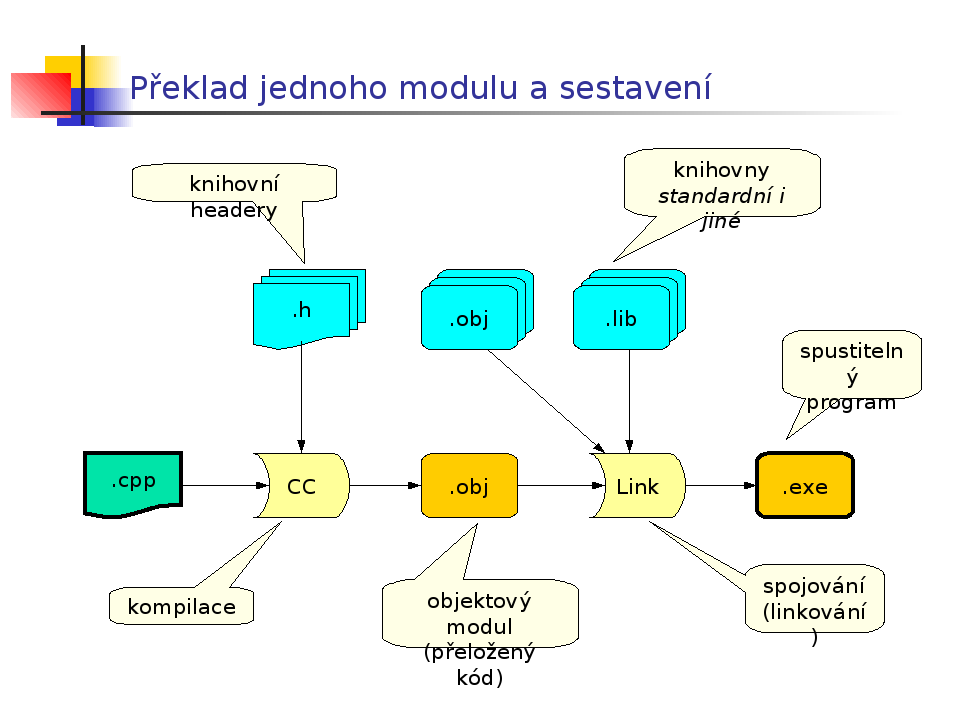
\includegraphics[width=10cm]{informatika/programovanie/obrazky/oddelenypreklad01.png}
\end{center}
\par\begin{center}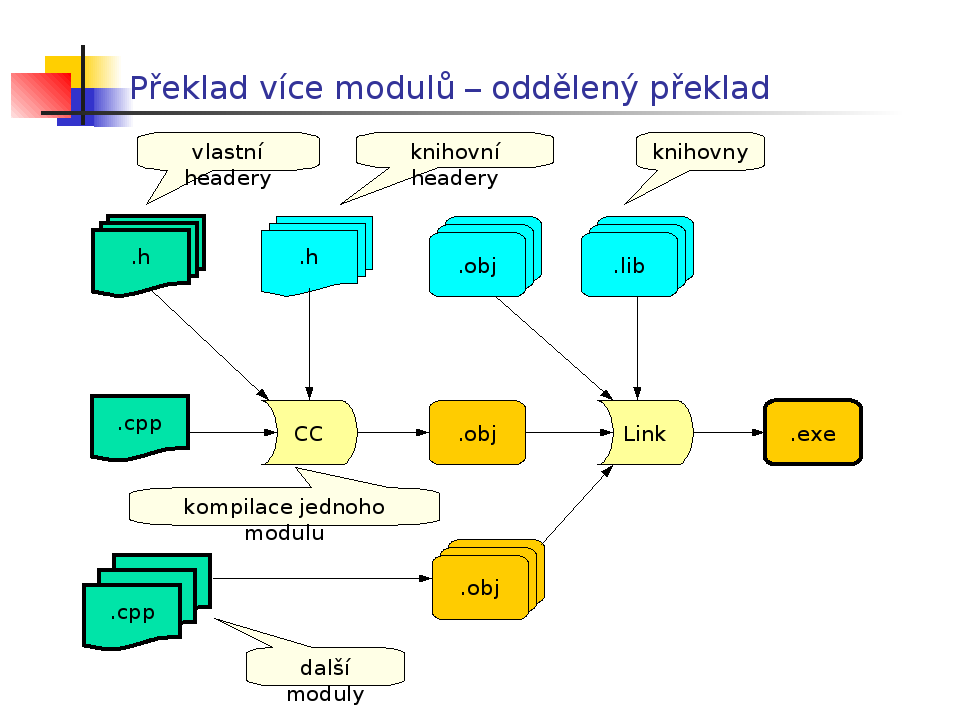
\includegraphics[width=10cm]{informatika/programovanie/obrazky/oddelenypreklad02.png}\end{center}
Smysl odděleného překladu modulů je urychlení celkového překladu -- nepřekládat to, co se od minula nezměnilo. Oddělený překlad dnes díky automatizaci makefily (viz níže) a integrovanými prostředími není téměř pro programátora vidět.

...pri tomto slide je vhodné ujasniť si, ako funguje statické a dynamické linkovanie (ako, kde a kedy sa opravujú adresy objektov atď.):
\begin{pitemize}
    \item \emph{Statické linkování} \\ Po odděleném překladu jednotlivé object moduly ještě neobsahují přímo adresy všech funkcí a externích identifikátorů, jen odkazy na ně. Linker se postará o jejich spojení dohromady. Je nutné, aby jména byla unikátní, takže u přetížených a virtuálních funkcí, jako je v C++, musí bý jména zpotvořena tak, aby ukazovala i třídu, namespace, parametry a jejich typy. To má na starosti compiler a říká se tomu \emph{name mangling}.
    \item \emph{Dynamické linkování} \\ Nastává po volání operačního systému -- zavedení dynamické knihovny do paměti. Jsou dvě možnosti jeho provedení, první je právě při zavádění knihovny, kdy se odkazy na všechny funkce (a mezi nimi navzájem) naplní správnými hodnotami (podle bázové adresy, na kterou se knihovna do paměti nahraje). Druhá možnost je použití dvou pointerů při volání funkcí z knihovny -- to se vytvoří tabulka skutečných adres, na kterou se z knihovny ukazuje. První možnost trvá déle při zavádění knihovny, druhá je zase pomalejší při provádění, ale umožňuje kód knihovny beze změn sdílet více procesy.
\end{pitemize}


\par\begin{center}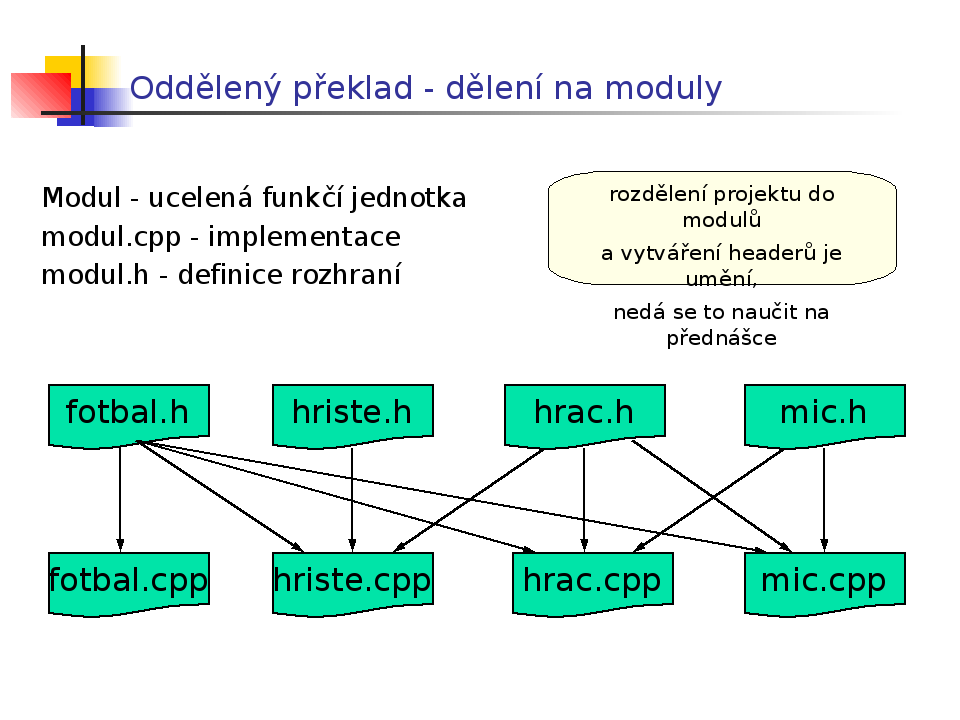
\includegraphics[width=10cm]{informatika/programovanie/obrazky/oddelenypreklad03.png}\end{center}

\emph{Linker} je program, který prijímá jeden alebo více objektů generovaných kompilátorem a složí je v jeden spustitelný program.

Objektový kód, nebo objektový soubor je reprezentace kódu, který kompilátor nebo assembler vytvoří zpracováním zdrojového kódu. Objektové soubory obsahují kompaktní kód, často nazývaný \uv{binárky} :-) Linker se typicky používá na vytvoření spustitelnýho souboru nebo knihovny spojením (slinkováním) objektových souborů. Základní častí objektového souboru je strojový kód (kód přimo vykonávaný CPU počítače).

\subsubsection*{Makefile}

Smyslem programu \emph{make} je řízení překladu a linkování. Popis závislostí jednotlivých modulů a hlavičkových na sobě je definován v 1 textovém souboru -- \emph{Makefile} (tj. které soubory je nutné mít aktuální/vytvořené pro překlad kterého souboru). Make vždy po změně souboru přeloží jen to, co na něm závisí.
Formát souboru make:
\begin{verbatim}
targets: files; 
        commands; #comment; line-begin\
        line contd.;
\end{verbatim}
Targets -- cíle činností / cílové soubory, možno definovat vic, při spuštění make bez parametrů se bere první; univ. nástroj (nejen pro překlad C/C++). Lze definovat i vlastní makra (příkazem \texttt{<název makra> = <string>}) a pak je používat (\texttt{\$\{makro\}}).
